% REMEMBER TO SET LANGUAGE!
\documentclass[a4paper,10pt,english]{article}
\usepackage[utf8]{inputenc}
%\usepackage[norsk]{babel}
% Standard stuff
\usepackage{amsmath,graphicx,varioref,verbatim,amsfonts,geometry,mathtools}
% colors in text
\usepackage{xcolor}
% Hyper refs
\usepackage[colorlinks]{hyperref}

% Document formatting
\setlength{\parindent}{0mm}
\setlength{\parskip}{1.5mm}

\usepackage[citestyle=phys]{biblatex}
\addbibresource{citations.bib}

%Color scheme for listings
\usepackage{textcomp}
\definecolor{listinggray}{gray}{0.9}
\definecolor{lbcolor}{rgb}{0.9,0.9,0.9}

%Listings configuration
\usepackage{listings}
%Hvis du bruker noe annet enn python, endre det her for å få riktig highlighting.
\lstset{
	backgroundcolor=\color{lbcolor},
	tabsize=4,
	rulecolor=,
	language=python,
        basicstyle=\scriptsize,
        upquote=true,
        aboveskip={1.5\baselineskip},
        columns=fixed,
	numbers=left,
        showstringspaces=false,
        extendedchars=true,
        breaklines=true,
        prebreak = \raisebox{0ex}[0ex][0ex]{\ensuremath{\hookleftarrow}},
        frame=single,
        showtabs=false,
        showspaces=false,
        showstringspaces=false,
        identifierstyle=\ttfamily,
        keywordstyle=\color[rgb]{0,0,1},
        commentstyle=\color[rgb]{0.133,0.545,0.133},
        stringstyle=\color[rgb]{0.627,0.126,0.941}
        }



%\renewcommand{\thesubsection}{\thesection.\alph{subsection}}

%\newcounter{subproject}
%\renewcommand{\thesubproject}{\alph{subproject}}
%\newenvironment{subproj}{
%\begin{description}
%\item[\refstepcounter{subproject}(\thesubproject)]
%}{\end{description}}

%Lettering instead of numbering in different layers
%\renewcommand{\labelenumi}{\alph{enumi}}
%\renewcommand{\thesubsection}{\alph{subsection}}

\newcommand{\Hh}{\prescript{1}{1}{H}}
\newcommand{\He}{\prescript{3}{2}{He}}

%opening
\title{AST3310 Project 1: Stellar Energy Production}
\author{Caspar William Bruenech}

\begin{document}

\maketitle

\section{Introduction}

 The energy produced by stars comes from the fusion of lighter elements into heavier isotopes. Due to the difference in atomic binding energy, energy is released as a result of the fusion. While there are many complicated processes making up the total energy production, the two main ones, for stars with sun-like core temperatures, are the so-called proton-proton-chain and CNO-cycle, who, respectively, fuse hydrogen into helium, and carbon, nitrogen and oxygen into helium. Both processes are made up of a series of branches, all of which are given in appendices \ref{appendix:PP} and \ref{appendix:CNO}. Using a theories about the nuclear reactions in the stellar core, combined with a variety of simplifications, we will in this experiment produce a numerical model for the stellar energy production, which hopefully will give us insight into how much energy is produced by the sun. We will be looking at the energy output from the various reactions by computing the mass difference as a result of the fusion process, followed by the energy production of the different branches of the reaction chains. Additionally, we will study how different temperatures of the core changes how much branches of the reactions chains contribute to the total energy production.

\section{Method}

\subsection{Energy Production and Reaction Rates}

 For the model to be designed in this project, we will be looking at the stellar energy production at one give point in time, and therefore ignoring the time-evolution of physical parameters, meaning that we will assume the mass fraction of the various elements remain constant throughout the fusion processes. The energy production is defined as how much energy is outputted per mass per second. As a result, we need to know not how often a certain reaction happens per mass. This is know as the reaction rate (per unit mass), and is defined as (\cite{Gudiksen2015})

$$r_{ik} = \frac{n_i n_k}{\rho(1 + \delta_{ik})} \lambda_{ik},$$

where $n_i$ is the number density of element $i$ with units $m^{-3}$,  $\rho$ is the stellar core mass density, $\delta_{ik}$ is the Kronecker-delta, and $\lambda_{ik}$ is the reaction rate \textit{not} per unit mass. The value of $\lambda$ for the relevant reactions in this experiment are given by \cite{Caughlan1988}.  

\subsection{The Proton-Proton (PP) Chain}

The reactions in the pp-chain are shown in appendix \ref{appendix:PP}. It consists of a total of 10 reactions spread over one main tree and three branches. The first two steps (hereby denoted as the $pp$-reaction) are common for all the three branches, while the road to producing helium-4 is divided into three possible routes. When computing the energy output of the various reactions in the pp-chain, we can make some approximations. Firstly, the first two reactions ($pp$), can be simplified to the fusion of three hydrogen-atoms to one helium-3 isotope. This is because the reaction time for the first reaction is of the order $10^{10} yr$, while the fusion of deuterium and hydrogen-1 happens within a few seconds (\cite{Gudiksen2015}), meaning we can approximate it as instantaneous in comparison. Thus the effective reaction becomes

$$\prescript{1}{1}{H} + \prescript{1}{1}{H} + \prescript{1}{1}{H} \rightarrow \prescript{3}{2}{He} + \nu_e.$$

Similarly, the pp-III-branch ends with two elementary decays, first $\prescript{8}{5}{B}$ to $\prescript{8}{4}{Be}$ and a neutrino, and then $\prescript{8}{4}{Be}$ to two $\prescript{4}{2}{He}$. These decays happen extremely fast, with the latter reaction having a half-life of $8.2\times 10^{-17}s$\cite{Gudiksen2015}, thus again becoming approximately instantaneous in comparison to the other reactions. Therefore, these days can be assumed to be a part of the $\prescript{7}{4}{Be} + \prescript{1}{1}{H}$-reaction (denoted $'17'$), such that it effectively becomes

$$\prescript{7}{4}{Be} + \prescript{1}{1}{H} \rightarrow 2\prescript{4}{2}{He} + \nu_e.$$

As a result, the reactions (and therefore changes in mass) and their corresponding reaction rates that we need to consider when calculating the energy production of the pp-chain are then:

All

$$\prescript{1}{1}{H} + \prescript{1}{1}{H} + \prescript{1}{1}{H} \rightarrow \prescript{3}{2}{He} + \nu_e \quad (pp),$$

pp-I,

$$\He + \He \rightarrow \prescript{4}{2}{He} + 2 \Hh \quad (33),$$

pp-II,

$$\He + \prescript{4}{2}{He} \rightarrow \prescript{7}{2}{Be} \quad (34),$$
$$\prescript{7}{4}{Be} + e^- \rightarrow \prescript{7}{3}{Li} + \nu_e \quad (e7),$$
$$\prescript{7}{3}{Li} + \Hh \rightarrow 2\prescript{4}{2}{He} \quad (17'),$$

pp-III,

$$\He + \prescript{4}{2}{He} \rightarrow \prescript{7}{4}{Be} \quad (17).$$
 
\subsection{The CNO Cycle}

As we see in appendix \ref{appendix:CNO}, the CNO cycle consists of a total of six steps. There are few things to note about this reaction chain; firstly, we observe that the entire process is essentially four hydrogen atoms producing one helium-4 isotope. This is because of the fact that all the elements produced in the various steps are all then utilized in the step directly following it, meaning they transmute into each other. As a result, the total energy output can be computed from the mass difference of four hydrogen atoms minus one helium-4 atom, minus the energy of the two neutrinos produced in step 2 and 5. However, we also need a reaction rate in order to compute the energy per mass per time. In order to compute this, we can approximate the reaction rate for the whole cycle with the reaction rate of the

$$\prescript{14}{7}{N} + \prescript{1}{1}{H} \rightarrow \prescript{15}{8}{O} + \gamma \quad (p14)$$

reaction by using the argument as used when approximating the reaction rate for the first two steps in the pp-chain, namely that the rate for this reaction is of several orders of magnitude larger than the other steps in the cycle (\cite{Gudiksen2015}), meaning that we can assume they happen instantaneously in comparison. Thus we can compute the total energy produced by the CNO-cycle as

$$E^{CNO} = \left[(4m_H - m_{\prescript{4}{2}{He}})\times c^2 - Q_{\nu_e}\right] \times r_{p14},$$

where $r_{p14}$ is the reaction rate for the above-mentioned reaction, and $Q_\nu$ is the sum of the neutrino energies for step 2 and 5 in the CNO cycle.

\subsection{Rescaling Reaction Rates}

In order to produce accurate results, we need to make sure that no reaction uses more of an element than is produced by a preceding reaction. This means we need to adjust the reaction rates. To do this, we can simply look at the reactions and note which ones requires the presence of an element which is produced by preceding reactions. We see that this is true for for the first reaction step, which produces hydrogen for the PP I branch and the first step of the PP II and PP III branches. By counting the number of hydrogen-3 isotopes required, we observe that we need to rescale the \textit{33}- and \textit{34}-reaction rates such that their sum is equal to the reaction rate for the \textit{pp}-reaction. I.e. we need to multiply them with the quantity 

$$a = \frac{r_{pp}}{2r_{33} + r_{34}},$$

which comes from the inequality criterion 

$$r_{pp} < a\times (2r_{33} + r_{34}).$$

The factor of 2 comes from the fact that two hydrogen-3 isotopes are used in the PP I branch. Next, we see that the beryllium-7 produced by the first steps of the PP II and PP III branches are used for the two following reactions in both branches. As a result, we introduce a test to check whether the reaction rate for the $34$-reaction, which produces the beryllium, is smaller than the sum of the reaction rates for $e7$ and $17$, who both require one beryllium-7 isotope. If this is true, we scale the $e7$- and $17$-reaction rates with a factor (derived from a similar inequality as above)

$$a = \frac{r_{35}}{r_{e7} + r_{17}},$$

which ensures that these two reactions do not use more beryllium-7 than has been produced by the $34$-reaction. Finally, we observe that the lithium used for step three of the PP II branch is produced by the $e7$-reactions, and we therefore set the reaction rate of the Lithium-hydrogen reaction ($17'$) to be equal to the $e7$ reaction rate. 


\subsection{Computing the Energy Produced by Each Reaction Chain}

With all the assumptions and approximations taken into account, we have a total of seven reactions all for which we need three parameters:

\begin{itemize}
    \item The mass difference in each reaction,
    \item the energy of the neutrinos (if any) produced in the reaction,
    \item the reaction rates for each reaction.
\end{itemize}

Additionally, we require the number densities of each relevant element, including the electron densities in the stellar core. This can be approximated using the mass fraction of the atomic species, the density of the core, and the atomic mass times the number of nucleons. I.e.

$$n_A = \frac{\rho A}{Zm_u},$$

where $n_A$ is the number density per unit volume of element A, $\rho$ is the density of the stellar core, $A$ is the mass fraction of the relevant isotope, $Z$ is the nucleon number for the molecule (number of protons and neutrons), and $m_u$ is atomic mass. To compute the electron density, we will assume that all elements are ionized, in addition to assuming that all the electrons come from the hydrogen- and helium atoms. Thus the electron density becomes

$$n_e = n_e^H + n_e^{He} = n_H + 2n_{He},$$

where in the last step we have utilized the assumption of fully ionized elements. We can then insert the equation for the number density we defined above

$$n_e = \frac{\rho X}{m_H} + \frac{2\rho Y}{m_{\prescript{4}{2}{He}} }  = \frac{\rho X}{m_u} + \frac{2\rho Y}{4m_u},$$

$$= \frac{\rho}{m_u}\left(X + \frac{1-X}{2}\right) = \frac{\rho(1 + X)}{2m_u}.$$

Where $X$ and $Y$ are, respectively, the mass fractions of hydrogen and helium. With the assumption that all the electrons come from only these two elements, we have used that $X + Y = 1$ in order to eliminate $Y$ from the equation. 

There are two quantities we are interested in; (1) the energy output of each reaction as a result of the mass difference from the fusion process, and (2) the energy production from each of the different branches in the process. Note we differentiate between the energy output and the energy production, wherein the output is simply the amount of energy that is released in one single reaction, denoted as $Q$, while the energy production is how much energy is generated by each reaction per mass per second, denoted as $E$. Thus, for (1), we use the mass-energy equivalence principle $Q = \Delta m c^2$ to compute the energy output as a result of the change in mass. Here we also need to subtract the energy contained in a neutrino which is potentially produced in the process, as this energy does not contribute to the energy pool of the sun. For (2), the general formula is to multiply $Q_{ik}$ for reaction $ik$ with the corresponding reaction rate $r_{ik}$, and for each branch, sum over the energies produced in the reactions taking place in that branch. However, since we have adjusted the reaction rates by rescaling them, this is something we can not do straightforwardly. What we have essentially done by this adjustment is to \textit{distribute} the reaction rates for the reactions that produce elements that are required in other reactions. For example, while the $pp$-reaction is common for all the pp-branches, it does not happen every time one of the individual branch reactions happen. Therefore, the energy produced by the $pp$-reaction has to be distributed between the different PP branches, which is precisely what we did by rescaling the reaction rate. Therefore, the energy produced by the \textit{PP I}-branch, is the energy \textit{output} from each of the reactions involved ($pp$ and $33$) multiplied by the reaction rate of the $33$-reaction, as this reaction rate now contains the reaction rate of the $pp$-reaction and the $33$-reaction as a result of the rescaling/distribution. Essentially, for all the branches, we need to determine the limiting reaction rate. We can do this by backtracking the reactions. For \textit{PP I}, the $33$ reaction depends on the $pp$-reaction, and thus the $33$-reaction is the limiting factor. For the second branch, we have a total of four reactions; $pp$, $34$, $e7$, and $17'$, wherein the $17'$ reaction depends on the Lithium-7 produced in the $e7$-reaction, the $e7$ reaction again depends on the Beryllium-7 produced in $34$, $34$ depends on the Helium-4 produced in $33$ and the Helium-3 produced in $pp$, and finally $34$ depends on the Helium-3 produced in $pp$. Thus, the limiting reaction for the whole branch in the $17'$-reaction. The same argument can be made to show that the limiting reaction rate for the third branch is $17$. Thus, the energy production for each branch of the PP-chain and the CNO cycle can be computed as

$$E^{PP-I} = (Q'_{pp} + Q'_{33}) \times r_{33},$$

$$E^{PP-II} = (Q'_{pp} + Q'_{34} + Q'_{e7} + Q'_{17'}) \times r_{17'},$$

$$E^{PP-III} = (Q'_{pp} + Q'_{34} + Q'_{17}) \times r_{17},$$

$$E^{CNO} = (Q'_{p14}) \times r_{p14},$$

where $Q'$ denotes the energy output from the reaction minus the energy of the potentially produced neutrino, and $r_{ik}$ is, as described in 2.1, is the reaction rate for reaction $ik$. To get accurate results, we need to consider the electron capture of beryllium-7 in reaction $e7$. As noted in \cite{Caughlan1988}, this reaction has an upper limit at temperatures smaller than $10^6 K$, given by

$$\lambda_{e7} \leq \frac{1.57\times 10^{-7}}{n_e N_A}$$

where $n_e$ is the electron density and $N_A$ is Avogadros number. To implement this, a simple if-test will be used to check whether the temperature is lower than $10^6$, in which case the reaction rate will be returned with the appropriate value.

We are also interested in observing how much of the energy output from each reaction is lost as a result of the neutrinos that escape. The energies for the neutrinos produced by the various reactions is shown in table \ref{tab:neutrino}. The neutrino loss (in percentage) for a branch $b$ is then simply calculated as

$$loss^b_\nu = \frac{Q^b_{\nu}}{\sum_{i,k} Q_{ik}}$$

where $Q^b_\nu$ is the sum of all neutrino energies produced in branch $b$, and $\sum_{i,k} Q_{ik}$ is the sum of the energy output from all reactions $i,k$ in branch $b$.

\begin{table}[]\centering
\begin{tabular}{ll}
Reaction  & Energy $Q_\nu$ {[}MeV{]} \\ \hline
$pp$      & 0.265                    \\
$e7$      & 0.815                    \\
$17(8)$   & 6.711                    \\
$p14(13)$ & 0.707                    \\
$p14(15)$ & 0.997                    \\ \hline
\end{tabular}
\caption{Different energies carried by the neutrinos produced in the different reactions. The parenthesis denotes the reaction wherein the neutrino is realistically produced, but due to merging certain reactions with others, we assume the neutrino to be produced by the reaction outside the parenthesis. Gathered from \cite{Gudiksen2015}.}
\label{tab:neutrino}
\end{table}

\section{Implementation \& Results}

All the atomic masses used for this experiment were gathered from \cite{Wang2017}. Additionally, we assumed mass fractions of

$$X = 0.7$$
$$Y_{\prescript{3}{2}{He}} = 10^{-10}, \qquad Y_{\prescript{4}{2}{He}} = 0.29$$
$$Z_{\prescript{7}{3}{Li}} = 10^{-7},\quad Z_{\prescript{7}{4}{Be}} = 10^{-7}, \quad Z_{\prescript{14}{7}{N}} = 10^{-11}.$$

Using solar parameter values of

$$\rho = 1.62\times 10^{5}\frac{kg}{m^3}, \quad T = 1.54\times 10^7 K,$$

we produced the results displayed in table \ref{tab:results}, where the error is the absolute relative error computed as

$$error = \frac{|E'^{true} - E'^{comp}|}{E'^{true}},$$

where $E'$ denotes the energy production multiplied by the density $\rho$. $E'^{true}$ is the value which has been pre-calculated as shown in \cite{Rouppe2020}, and $E'^{comp}$ is the computed equivalent energy production.

\begin{table}[]\centering
\begin{tabular}{|l|l|l|l|l|}
\hline
                & Energy Output Q {[}$MeV${]} & Energy Produced E {[}$MeV/kgs${]} & Neutrino loss {[}\%{]} &  Error {[}\%{]} \\ \hline
$pp$            & 6.935                        &                   &                        & 10.05                             \\ \hline
$33$            & 12.86                        &                      &                        & 2.76                             \\ \hline
\textbf{PP I}   &                        & 0.522                  & 2.68                   &                                  \\ \hline
$34$            & 1.587                    &                   &                        & 0.19                             \\ \hline
$e7$            & 0.861                    &                     &                        & 3.91                             \\ \hline
$17'$          & 17.35                     &                  &                        & 0.14                             \\ \hline
\textbf{PP II}  &                         & 30179                  & 4.04                   &                                  \\ \hline
$17$            & 18.21                    &                   &                        & 0.07                             \\ \hline
\textbf{PP III} &                         & 107.8                  & 26.01                  &                                  \\ \hline
$p14$           & 26.73                    &                      &                        & 4.56                             \\ \hline
\textbf{CNO}    &                     & 3.698                     & 7.37                   &                                  \\ \hline
\end{tabular}
\label{tab:results}
\caption{The results of the computation using solar parameter values.}
\end{table}

By summing the energies produced by all the branches, we can compute the total energy production in the solar core, and the contribution to this energy pool from each branch. The result of this is shown in table \ref{tab:percent}.

\begin{table}[]\centering
\begin{tabular}{ll}
Branch   & Contribution {[}\%{]} \\ \hline
pp-I   & 0.002                 \\
pp-II  & 99.637                \\
pp-III & 0.349                 \\
CNO    & 0.012                 \\ \hline
\end{tabular}
\caption{The contribution of each reaction branch to the total energy production of the solar core.}
\label{tab:percent}
\end{table}

Using a temperature range of $T \in [10^4, 10^9]$, the energy production from each reaction chain for each temperature value was computed and plotted. The resulting figure is shown in figure \ref{fig:energy_temp}.

\begin{figure}
    \centering
    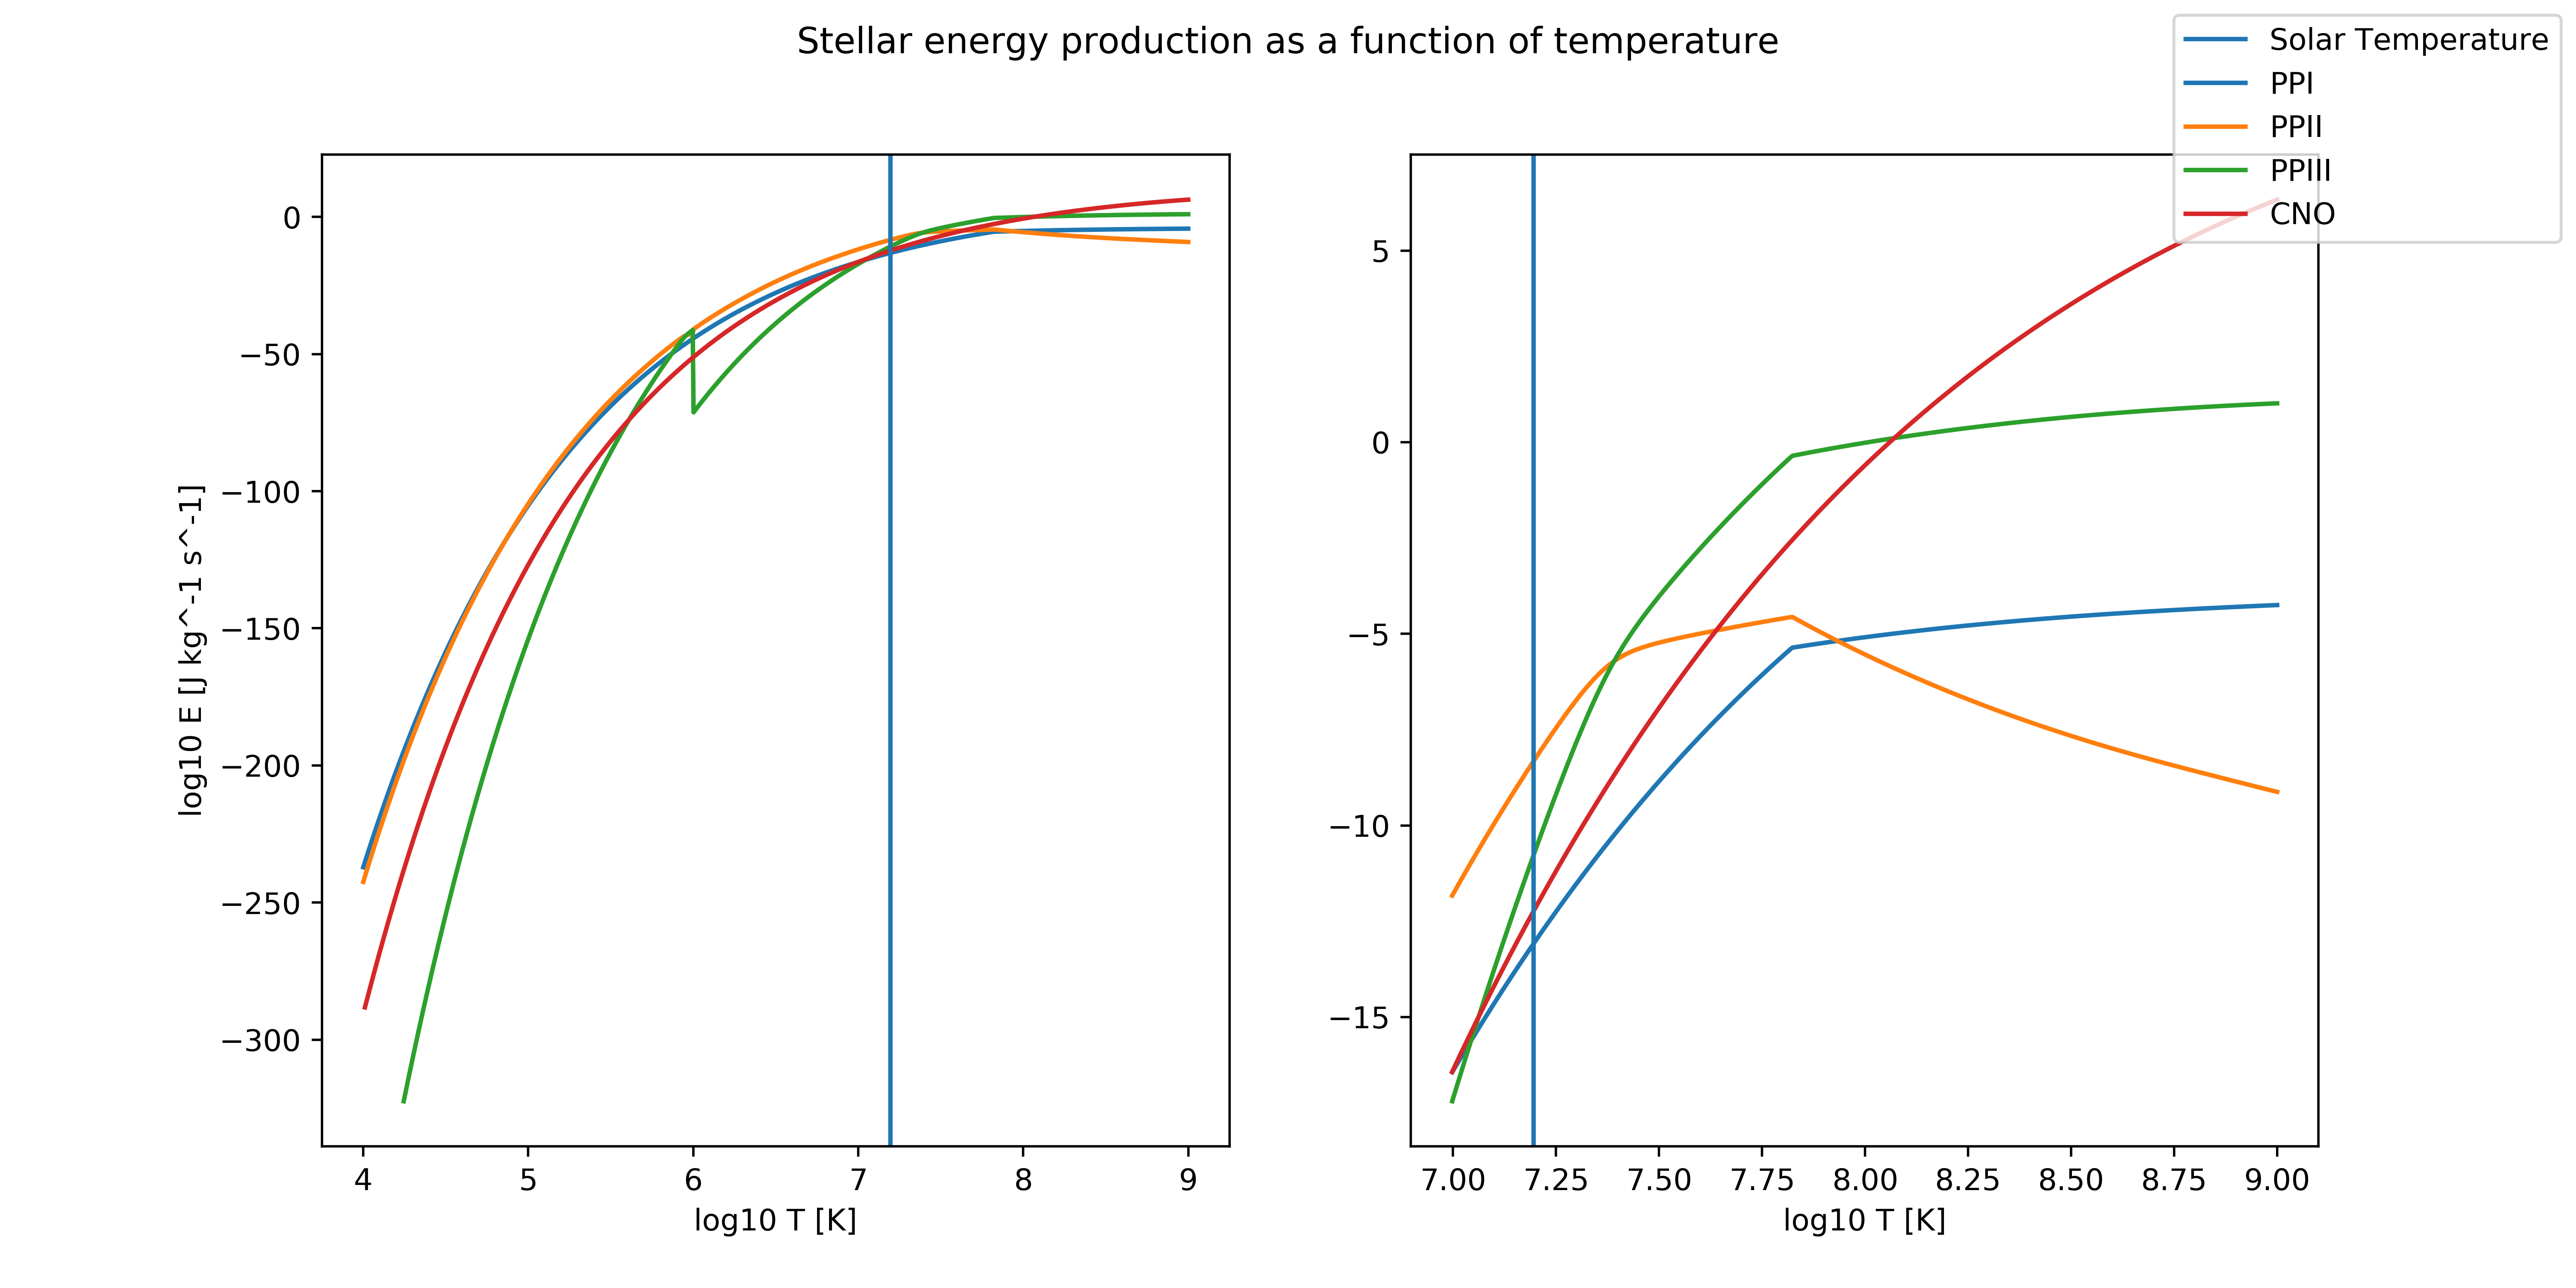
\includegraphics[width=1\textwidth]{energy_temperature.png}
    \caption{Caption}
    \label{fig:energy_temp}
\end{figure}

\section{Discussion}

The results of the energy output from the different reactions in table \ref{tab:results} are identical or significantly similar to the equivalent values that have been previously calculated in \cite{Gudiksen2015}, however there is a significant error in some of the reactions, specifically the $pp$, $e7$, and $p14$ reactions. Since the energy output is correct, the only possibility of the source of the error is in the reaction rate $r$, as the error is computed with the quantity $r_{ik}Q_{ik}\rho$. However, no such error was discovered in the value of $r$ for these reactions, and the source of the error was not found. 

The neutrino loss calculations show that the pp-III branch loses, with a strong margin, the most energy from neutrinos that escape the stellar core, with over a quarter of the energy lost. This is the result of the $\beta$-decay of boron-8, which produces very high energy neutrinos. We also observe that the CNO cycle requires the presence of carbon-12 to begin the process, an isotope which is not produced by any of the other reactions. In fact, carbon-12 is produced in the triple-alpha energy chain, which is only present in very high temperature stars. The carbon-12 in stars with sun-like temperatures then comes from the death of heavier stars, who produced carbon-12 in the triple-alpha process before ending in a supernova and ejecting their outer layers containing the carbon.

In table \ref{tab:percent} we see how the different branches/chains contribute to the total energy production of the solar core. We observe that the vast majority of the energy comes from the pp-II branch, while all the other chains all contributing with less than $1\%$, with $pp-I$ being the lowest of them all. It should be noted that the reactions in the CNO cycle utilized in this experiment are not all the reaction in the true CNO cycle, where in reality, the cycle contains a number of sub-branches. However, in the sun, these branches only contribute to about $0.05\%$ \cite{Gudiksen2015} of the total energy production. Also according to \cite{Gudiksen2015}, the CNO cycle should contribute with about $1.7\%$ of the total energy production. Since we are looking at the part which produces $99.5\%$ of the total CNO energy, we would expect to see CNO contribute with around $1.6915\%$, or $141$ times what we observed in the experiments. The reason for this substantial difference is most likely a result of the numerous approximations and simplifications we have included in our model, and as a result the values produced by this model should not be interpreted as being realistic. 

Nevertheless, we can still make some interesting observations from the produced data. Looking at the plot in figure \ref{fig:energy_temp}, we see that, as expected, the CNO cycle contributes with the smallest energy production in lower temperature stars, before eventually reaching the pp chain at $T \approx 10^7$ and overtaking it at temperatures $T \geq 10^8 K$. This is expected because the CNO cycle has a steeper incline as a function of temperature, and according to \cite{Schuler2009}, it becomes dominant at temperatures of around $T \approx 1.7 \times 10^7 K$. The figure also shows how the energy production of the pp-III branch has a sudden decrease at $T=10^6K$. This is the result of the constraint we put on the reaction rate for the $e7$ reaction due to the upper limit of the beryllium-7 electron capture for temperatures lower than $10^6 K$. When this kicks in, the reaction rate spikes, which causes more of the beryllium-7 to be used in the pp-II branch, where the $e7$-reaction takes place, thus reducing the amount available for reaction $17$ in the pp-III chain, which again reduces the energy production of this branch. 
At the solar temperature of $T = 1.56\times 10^7 K$, marked by the blue vertical line in the figure, we see that the majority of the energy comes from the pp-II branch, followed sequentially by pp-III, CNO and pp-I. This follows the values we computed in table \ref{tab:percent}. While the figure shows the interesting result of how the CNO cycle produces most of the energy in the hotter stars, the values for the energy production is not in line with more realistic models. One of the reasons for this is the fact that we used the same density ($\rho_{sun}$) for all the different temperature values. In reality, the density of the stellar core would most likely vary greatly for bigger stars with hotter cores.

To make the model more realistic, certain assumptions and simplifications can be omitted to produce a more complex and accurate model. Examples of this include using the true isotope mass when computing the number densities, instead of the nucleon number multiplied by the atomic mass, the electron density can be computed using the number densities of all the elements present, instead of assuming all the electrons come from only hydrogen and helium. Additionally, the core density can be created as a function of temperature to create more realistic models for the energy production of stars with temperatures different than the solar core temperature.

\section{Conclusion}

In this experiment we have created a numerical model for the energy production in a stellar core using a number of approximations and simplifications. With estimated core temperature and density from the sun, we calculated a total energy production contribution from the various branches in the pp-chain and CNO cycle. The result showed a macro view which was in line with real observations, in that CNO cycle contributed significantly less than the pp-chain. However, the details of the numbers do not add up with what has been previously computed by other sources, which is not surprising considering the amount of assumptions and simplifications we implemented into the model. Additionally, we observed how the various branches lose energy as a result of neutrinos that are produced in the reactions, but who do not contribute to the energy pool. It was found that the pp-III branch loses most of its energy, over a quarter, while the other branches were all under $10\%$. This was found to be due to the high energy neutrinos produced in the $\beta$-decay of boron-8. Finally, we observed how the different branches contribute to the energy pool as a function of the core temperature, and found, as was to be expected, that the pp-chain dominates the energy production in stars with temperatures below $\approx 10^{7,5}$, before being overtaken by the CNO cycle for higher temperatures. Again, the specific energy values are not to be taken as realistic, but the general behaviour did end up being in line with previous observations. 

Problems were encountered in the making of the numerical model, in that some reactions returned significant error rates, the cause of which was not found. Additionally, difficulties were found in justifying some of the simplifications that were made in the model, such as the use of nucleon number times atomic mass when computing the number densities. Nevertheless, we have learned how the various energy processes produce the energy in the stellar core, and how these vary with temperature.


\newpage

\appendix

\section{PP-Chain} \label{appendix:PP}

All steps:

$$\Hh + \Hh \rightarrow \prescript{2}{1}{D} + e^+ + \nu_e + \gamma$$
$$\prescript{2}{1}{D} + \Hh \rightarrow \prescript{3}{2}{He} + \gamma$$

PP I branch

$$\He + \He \rightarrow \prescript{4}{2}{He} + 2 \Hh + \gamma$$

PP II branch

$$\He + \prescript{4}{2}{He} \rightarrow \prescript{7}{2}{Be} + \gamma $$
$$\prescript{7}{4}{Be} + e^- \rightarrow \prescript{7}{3}{Li} + \nu_e + \delta E$$
$$\prescript{7}{3}{Li} + \Hh \rightarrow 2\prescript{4}{2}{He} + \gamma $$

PP III branch

$$\He + \prescript{4}{2}{He} \rightarrow \prescript{7}{4}{Be} + \gamma $$
$$\prescript{7}{4}{Be} + \Hh \rightarrow \prescript{8}{5}{B} + \gamma$$
$$\prescript{8}{5}{B} \rightarrow \prescript{8}{4}{Be} + e^+ + \nu_e + \gamma$$
$$\prescript{8}{4}{Be} \rightarrow 2\prescript{4}{2}{He} + \gamma $$

\section{CNO cycle} \label{appendix:CNO}

$$\prescript{12}{6}{C} + \Hh \rightarrow \prescript{13}{7}{N} + \gamma $$
$$\prescript{13}{7}{N} \rightarrow \prescript{13}{6}{C} + e^+ + \nu_e + \gamma$$
$$\prescript{13}{6}{C} + \Hh \rightarrow \prescript{14}{7}{N} + \gamma $$
$$\prescript{14}{7}{N} + \Hh \rightarrow \prescript{15}{8}{O} + \gamma $$
$$\prescript{15}{8}{O} \rightarrow \prescript{15}{7}{N} + e^+ + \nu_e + \gamma$$
$$\prescript{15}{7}{N} + \Hh \rightarrow \prescript{12}{6}{C} + \prescript{4}{2}{He} + \gamma $$

\printbibliography

\end{document}
